% -*- TeX-engine: xetex;  -*-
\documentclass[
letterpaper, % Stock and paper size.
11pt, % Type size.
% article,
oneside, 
onecolumn, % Only one column of text on a page.
% openright, % Each chapter will start on a recto page.
% openleft, % Each chapter will start on a verso page.
openany, % A chapter may start on either a recto or verso page.
]{memoir}

%%% PACKAGES 
%%%------------------------------------------------------------------------------

%\usepackage[utf8]{inputenc} % Not needed with XeTeX
\usepackage[T1]{fontenc}    %
\usepackage[english]{babel} % English please
\usepackage[final]{microtype} % Less badboxes

%\usepackage{amsmath,amssymb,mathtools} % Math

\usepackage{newtxtext}
\usepackage{newtxmath}
% \usepackage[libertine]{newtxtext}
% \usepackage[libertine]{newtxmath}
%\usepackage{dutchcal} % For lower-case calligraphic
\usepackage{BOONDOX-calo} % For lower-case calligraphic
\usepackage{pstricks,pst-node,pstricks-add}
\usepackage{multido}
\usepackage{url}
\usepackage[small,bf]{caption}
%\usepackage[dvips]{graphicx} % Include figures
\usepackage{siunitx}
\usepackage{enumitem}
\usepackage{graphicx}
%%% PAGE LAYOUT 
%%%------------------------------------------------------------------------------

\setlrmarginsandblock{0.15\paperwidth}{*}{1} % Left and right margin
\setulmarginsandblock{0.2\paperwidth}{*}{1}  % Upper and lower margin
\checkandfixthelayout

%%% SECTIONAL DIVISIONS
%%%------------------------------------------------------------------------------

\maxsecnumdepth{subsection} % Subsections (and higher) are numbered
\setsecnumdepth{subsection}

\makeatletter %
\makechapterstyle{standard}{
  \setlength{\beforechapskip}{0\baselineskip}
  \setlength{\midchapskip}{1\baselineskip}
  \setlength{\afterchapskip}{8\baselineskip}
  \renewcommand{\chapterheadstart}{\vspace*{\beforechapskip}}
  \renewcommand{\chapnamefont}{\centering\normalfont\Large}
  \renewcommand{\printchaptername}{\chapnamefont \@chapapp}
  \renewcommand{\chapternamenum}{\space}
  \renewcommand{\chapnumfont}{\normalfont\Large}
  \renewcommand{\printchapternum}{\chapnumfont \thechapter}
  \renewcommand{\afterchapternum}{\par\nobreak\vskip \midchapskip}
  \renewcommand{\printchapternonum}{\vspace*{\midchapskip}\vspace*{5mm}}
  \renewcommand{\chaptitlefont}{\centering\bfseries\LARGE}
  \renewcommand{\printchaptertitle}[1]{\chaptitlefont ##1}
  \renewcommand{\afterchaptertitle}{\par\nobreak\vskip \afterchapskip}
}
\makeatother

\chapterstyle{standard}

\setsecheadstyle{\normalfont\large\bfseries}
\setsubsecheadstyle{\normalfont\normalsize\bfseries}
\setparaheadstyle{\normalfont\normalsize\bfseries}
\setparaindent{0pt}\setafterparaskip{-1em}

%%% FLOATS AND CAPTIONS
%%%------------------------------------------------------------------------------

\makeatletter                  % You do not need to write [htpb] all the time
\renewcommand\fps@figure{htbp} %
\renewcommand\fps@table{htbp}  %
\makeatother                   %

\captiondelim{\space } % A space between caption name and text
\captionnamefont{\small\bfseries} % Font of the caption name
\captiontitlefont{\small\normalfont} % Font of the caption text

%\changecaptionwidth          % Change the width of the caption
%\captionwidth{1\textwidth} %

%%% ABSTRACT
%%%------------------------------------------------------------------------------

\renewcommand{\abstractnamefont}{\normalfont\small\bfseries} % Font of abstract title
\setlength{\absleftindent}{0.1\textwidth} % Width of abstract
\setlength{\absrightindent}{\absleftindent}

%%% HEADER AND FOOTER 
%%%------------------------------------------------------------------------------

\makepagestyle{standard} % Make standard pagestyle

\makeatletter                 % Define standard pagestyle
\makeevenfoot{standard}{}{}{} %
\makeoddfoot{standard}{}{}{}  %
\makeevenhead{standard}{\bfseries\thepage\normalfont\qquad\small\leftmark}{}{}
\makeoddhead{standard}{}{}{\small\rightmark\qquad\bfseries\thepage}
% \makeheadrule{standard}{\textwidth}{\normalrulethickness}
\makeatother                  %

\makeatletter
\makepsmarks{standard}{
\createmark{chapter}{both}{shownumber}{\@chapapp\ }{ \quad }
\createmark{section}{right}{shownumber}{}{ \quad }
\createplainmark{toc}{both}{\contentsname}
\createplainmark{lof}{both}{\listfigurename}
\createplainmark{lot}{both}{\listtablename}
\createplainmark{bib}{both}{\bibname}
\createplainmark{index}{both}{\indexname}
\createplainmark{glossary}{both}{\glossaryname}
}
\makeatother                               %

\makepagestyle{chap} % Make new chapter pagestyle

\makeatletter
\makeevenfoot{chap}{}{\small\bfseries\thepage}{} % Define new chapter pagestyle
\makeoddfoot{chap}{}{\small\bfseries\thepage}{}  %
\makeevenhead{chap}{}{}{}   %
\makeoddhead{chap}{}{}{}    %
% \makeheadrule{chap}{\textwidth}{\normalrulethickness}
\makeatother

\nouppercaseheads
\pagestyle{standard}               % Choosing pagestyle and chapter pagestyle
\aliaspagestyle{chapter}{chap} %

%%% NEW COMMANDS
%%%------------------------------------------------------------------------------


%%% TABLE OF CONTENTS
%%%------------------------------------------------------------------------------

\maxtocdepth{subsection} % Only parts, chapters and sections in the table of contents
\settocdepth{subsection}

\AtEndDocument{\addtocontents{toc}{\par}} % Add a \par to the end of the TOC


% Use amsmath (already included by newtx packages)
% commands to make equations and figures be numbered within chapters: 
\numberwithin{equation}{chapter}
\numberwithin{figure}{chapter}
\renewcommand{\theequation}{\arabic{chapter}.\arabic{equation}}
\renewcommand{\thefigure}{\arabic{chapter}.\arabic{figure}}


%%% INTERNAL HYPERLINKS
%%%-------------------------------------------------------------------------------

\usepackage{hyperref}   % Internal hyperlinks
\hypersetup{
pdfborder={0 0 0},      % No borders around internal hyperlinks
pdfauthor={Peter S. Simon} % author
}
\usepackage{memhfixc}   %

%%% THE DOCUMENT
%%% Where all the important stuff is included!
%%%-------------------------------------------------------------------------------

\author{Peter S. Simon}
\title{PSSFSS Theory Documentation}

%%%%%%%%%%%%%%%%%%%%%% Begin macro definitions  %%%%%%%%%%%%%%%%%%%%%%%%%%%%%%%
%\usepackage{bm} % Correct bold math
\newcommand{\pssfss}{PSSFSS}
\renewcommand{\d}{\text{d}}  % for use in integrals
\newcommand{\Realnum}{\mathbb{R}}
\newcommand{\Complexnum}{\mathbb{C}}
\newcommand{\Integers}{\mathbb{Z}}
\newcommand{\Fourier}{\mathcal{F}}
\DeclareMathOperator{\RealOp}{Re}
\DeclareMathOperator{\sgn}{sgn}
\newcommand{\Real}[1]{\RealOp\left\{#1\right\}}
\DeclareMathOperator{\ImagOp}{Im}
\newcommand{\Imag}[1]{\ImagOp\left\{#1\right\}}
\newcommand{\diag}[1]{\text{diag}\left\{#1\right\}}
\newcommand{\0}{\boldsymbol{0}}
\newcommand{\A}{\boldsymbol{A}}
\newcommand{\E}{\boldsymbol{E}}
\newcommand{\e}{\boldsymbol{e}}
\renewcommand{\k}{\boldsymbol{k}}
\newcommand{\f}{\boldsymbol{f}}  % Basis function.
\newcommand{\ftf}{\boldsymbol{\tilde{f}}}  % Basis function Fourier transform.
\newcommand{\F}{\boldsymbol{F}}
\renewcommand{\H}{\boldsymbol{H}}
\newcommand{\h}{\boldsymbol{h}}
\newcommand{\rhat}{\boldsymbol{\hat{r}}}
\newcommand{\thetahat}{\boldsymbol{\hat{\theta}}}
\newcommand{\phihat}{\boldsymbol{\hat{\phi}}}
\newcommand{\hhat}{\rlap{$\boldsymbol{\hat{h}}$}\phantom{\boldsymbol{h}}}
\newcommand{\vhat}{\rlap{$\boldsymbol{\hat{v}}$}\phantom{\boldsymbol{v}}}
\newcommand{\Rhat}{\boldsymbol{\hat{R}}}
\newcommand{\Lhat}{\boldsymbol{\hat{L}}}
\newcommand{\J}{\boldsymbol{J}}
\newcommand{\Jt}{\boldsymbol{\tilde{J}}}
\newcommand{\I}{\boldsymbol{I}}
\newcommand{\K}{\boldsymbol{K}}
\newcommand{\Js}{\J_{\text{s}}}
\newcommand{\ftJs}{\boldsymbol{\tilde{J}}_{\text{s}}}
\renewcommand{\L}{\boldsymbol{L}}
\newcommand{\M}{\boldsymbol{M}}
\newcommand{\Ms}{\boldsymbol{M}_{\text{s}}}
\newcommand{\ftMs}{\boldsymbol{\tilde{M}}_{\text{s}}}
\renewcommand{\r}{\boldsymbol{r}}
\newcommand{\x}{\boldsymbol{\hat{x}}}
\newcommand{\y}{\boldsymbol{\hat{y}}}
\newcommand{\z}{\boldsymbol{\hat{z}}}
\newcommand{\abs}[1]{\lvert#1\rvert}
\newcommand{\norm}[1]{\left\lVert#1\right\rVert}
\newcommand{\gradient}{\boldsymbol{\nabla}}
\newcommand{\cross}{\boldsymbol{\times}}
\newcommand{\bdot}{\boldsymbol{\cdot}}
\newcommand{\curl}{\boldsymbol{\nabla} \cross}
\newcommand{\divergence}{\boldsymbol{\nabla} \bdot}
\newcommand{\laplace}{\nabla^2}  % Scalar Laplacian Operator
\newcommand{\vlaplace}{\gradient^2}  % Vector Laplacian Operator
\newcommand{\qe}{q_{\text{e}}}  % Electric charge density
\newcommand{\qm}{q_{\text{m}}}  % Magnetic charge density
\newcommand{\union}{\bigcup}  % Magnetic charge density
\newcommand{\s}{\boldsymbol{s}}  % Direct lattice vector
\newcommand{\vecbeta}{\boldsymbol{\beta}}  % Reciprocal lattice vector
\newcommand{\betahat}{\boldsymbol{\hat{\beta}}}  % Reciprocal lattice unit vector
\newcommand{\vecrho}{\boldsymbol{\rho}}  % Reciprocal lattice vector
\newcommand{\colvec}[1]{\begin{bmatrix} #1 \end{bmatrix}}
%\newcommand{\colvec}[1]{\left[\begin{array}{c} #1 \end{array}\right]}
\newcommand{\TE}{^{\text{TE}}}
\newcommand{\TM}{^{\text{TM}}}
\newcommand{\mat}[1]{\boldsymbol{\mathcal{#1}}}
\newcommand{\matel}[1]{\mathcal{#1}}
\newcommand{\Icoef}{\matel{I}}  % Electric current expansion coefficient.
\newcommand{\Vcoef}{\matel{V}}  % Magnetic current expansion coefficient.
\newcommand{\one}{^{(1)}} % Region 1 designator
\newcommand{\two}{^{(2)}} % Region 2 designator
\newcommand{\eye}{^{(i)}} % Region i designator
\newcommand{\epw}{^{(i+1)}} % Region i+1 designator
\newcommand{\enn}{^{(N)}} % Region N designator
\newcommand{\ess}{^{(s)}} % Region s designator
\newcommand{\spw}{^{(s+1)}} % Region s+1 designator
\newcommand{\tmi}{^{(3-i)}} % Region 3-i designator
\newcommand{\three}{^{(3)}} % Region 3 designator
\newcommand{\four}{^{(4)}} % Region 4 designator
\newcommand{\transpose}{^{\text{\sffamily{T}}}}
\newcommand{\hermitian}{^{\text{\sffamily{H}}}}
\newcommand{\inc}{^{\text{inc}}}
\newcommand{\refl}{^{\text{ref}}}
\newcommand{\trans}{^{\text{tran}}}
\newcommand{\scat}{^{\text{sc}}}
\renewcommand{\t}{\boldsymbol{\hat{t}}}
\newcommand{\n}{\boldsymbol{\hat{n}}}
\newcommand{\pdx}[1]{\frac{\partial #1}{\partial x}}
\newcommand{\pdz}[1]{\frac{\partial #1}{\partial z}}
\newcommand{\pdu}[1]{\frac{\partial #1}{\partial u}}
\newcommand{\summn}{\sum_{m,n}}
\newcommand{\dyad}[1]{\boldsymbol{\bar{#1}}}
\newcommand{\Idemfactor}{\dyad{I}}
\newcommand{\GAxx}{G^A_{xx}}
\newcommand{\GtAxx}{\tilde{G}^{A}_{xx}}
\newcommand{\GFxx}{G^F_{xx}}
\newcommand{\GrFxx}{\raisebox{0pt}[0pt][0pt]{$\vecr{G}$}\vphantom{G}^F_{xx}}
\newcommand{\GlFxx}{\raisebox{0pt}[0pt][0pt]{$\vecl{G}$}\vphantom{G}^F_{xx}}
\newcommand{\GPhi}{{G}^{\Phi}}
\newcommand{\GtPhi}{{G}^{\Phi}}
\newcommand{\GPsi}{{G}^{\Psi}}
\newcommand{\GrPsi}{\raisebox{0pt}[0pt][0pt]{$\vecr{G}$}\vphantom{G}^\Psi}
\newcommand{\GlPsi}{\raisebox{0pt}[0pt][0pt]{$\vecl{G}$}\vphantom{G}^\Psi}
\newcommand{\rcp}{\r^{\text{c}+}} % Positive centroid r vector.
\newcommand{\rcm}{\r^{\text{c}-}} % Negative centroid r vector.
\newcommand{\rcpm}{\r^{\text{c}\pm}} % Plus or Negative centroid r vector.
\newcommand{\vecrhocp}{\vecrho^{\text{c}+}} % Positive centroid rho vector.
\newcommand{\vecrhocm}{\vecrho^{\text{c}-}} % Positive centroid rho vector.
\newcommand{\vecrhocpm}{\vecrho^{\text{c}\pm}} % Positive centroid rho vector.
\newcommand{\innerprod}[1]{\left< #1 \right>}
%\renewcommand{\iint}{\int \!\!\! \int}
\newcommand{\rcu}{\r^{\text{c}u}} % Centroid r vector for triangle ``u''.
\newcommand{\rhocu}{\rho^{\text{c}u}} % Centroid rho for triangle ``u''.
\renewcommand{\P}{\boldsymbol{P}}
\renewcommand{\l}{\boldsymbol{l}}
\newcommand{\lhat}{\boldsymbol{\hat{l}}}
\renewcommand{\u}{\boldsymbol{\hat{u}}}  % unit vector.
\newcommand{\is}{i_{\text{s}}}  % Source region designator
\renewcommand{\it}{i_{\text{t}}}  % Transmitted region designator
\newcommand{\eyes}{^{(\is)}} % Source Region designator
\newcommand{\eyet}{^{(\it)}} % Transmitted Region designator
% Vector accent pointing to left:
\newcommand{\vecl}[1]{\overset{\raisebox{-0.6ex}{\tiny$\boldsymbol{\leftarrow}$}}{#1}}  
% Vector accent pointing to right:
\newcommand{\vecr}[1]{\overset{\raisebox{-0.6ex}{\tiny$\mkern5mu\boldsymbol{\rightarrow}$}}{#1}}  
\newcommand{\Zright}{\vecr{Z}}
\newcommand{\Zleft}{\vecl{Z}}
%\newcommand{\Yleft}{\vecl{Y}}
%\newcommand{\Yright}{\vecr{Y}}
 \newcommand{\Yleft}%
     {\raisebox{0pt}[0pt][0pt]{\rlap{$\vecl{\phantom{Y}}$}}Y}  % TLGF
 \newcommand{\Yright}%
 {\raisebox{0pt}[0pt][0pt]{\rlap{$\vecr{\phantom{Y}}$}}Y}  % TLGF
\newcommand{\Vi}{V_{\text{i}}}  % TLGF
\newcommand{\Vv}{V_{\text{v}}}  % TLGF
\newcommand{\Ii}{I_{\text{i}}}  % TLGF
\newcommand{\Iv}{I_{\text{v}}}  % TLGF

 \newcommand{\Ilv}%
 {\raisebox{0pt}[0pt][0pt]{\rlap{$\vecl{I}$}}\phantom{I}_{\text{v}}}  % TLGF
 \newcommand{\Irv}%
 {\raisebox{0pt}[0pt][0pt]{\rlap{$\vecr{I}$}}\phantom{I}_{\text{v}}}  % TLGF
\newcommand{\tauhat}%
 {\rlap{$\boldsymbol{\hat{\tau}}$}\phantom{\boldsymbol{\tau}}} % Pol. vector
%\newcommand{\sigmahat}{\boldsymbol{\hat{\sigma}}}  % Polarization vector
\newcommand{\uhat}{\boldsymbol{\hat{u}}}  % Polarization vector
\newcommand{\what}{\boldsymbol{\hat{w}}}  % Polarization vector
\newcommand{\khat}{\boldsymbol{\hat{k}}}  % Polarization vector
\newcommand{\sigmahat}%
 {\rlap{$\boldsymbol{\hat{\sigma}}$}\phantom{\boldsymbol{\sigma}}} % Pol. vec.
\newcommand{\piotwo}{{\textstyle\frac{\pi}{2}}}

%% \tlsection{x1}{x4}{n} draws a transmission line section
%% from x1 to x4, with nodes at x1 and x4, and labels the 
%% section as number ``n''
\newcommand{\tlsection}[3]{%
                                % Draw top line:
  \mmultido{\rrone=#1+0.3,\rrtwo=#2+-0.3}{1}{%
    \qdisk(#1,0.8){1.5pt} \psline(#1,.8)(\rrone,.8) %
    \psframe(\rrone,0.7)(\rrtwo,0.9) %
    \psline(\rrtwo,0.8)(#2,0.8) \qdisk(#2,0.8){1.5pt} %
                                % Draw bottom line
    \qdisk(#1,-0.8){1.5pt} \psline(#1,-0.8)(\rrone,-0.8) %
    \psframe(\rrone,-0.9)(\rrtwo,-0.7) %
    \psline(\rrtwo,-0.8)(#2,-0.8) \qdisk(#2,-0.8){1.5pt} %
                                % Labels
    \pcline[linestyle=none](\rrone,0)(\rrtwo,0)
    \lput{:U}{\cstack{$Z_{pmn}^{(#3)}$ \\[0.5ex] $\gamma_{mn}^{(#3)}$}}
                                % Dimensions
    \pcline[linewidth=0.5pt]{<->}(\rrone,1.3)(\rrtwo,1.3)
    \pcline{|-|}(\rrone,1.3)(\rrtwo,1.3)
    \lput*{:U}{$h^{(#3)}$}
    }
  }

%% \Ytlsection{x1}{x4}{n} draws a transmission line section
%% from x1 to x4, with nodes at x1 and x4, and labels the 
%% section as number ``n'' using a Y rather than a Z
\newcommand{\Ytlsection}[3]{%
                                % Draw top line:
  \mmultido{\rrone=#1+0.3,\rrtwo=#2+-0.3}{1}{%
    \qdisk(#1,0.8){1.5pt} \psline(#1,.8)(\rrone,.8) %
    \psframe(\rrone,0.7)(\rrtwo,0.9) %
    \psline(\rrtwo,0.8)(#2,0.8) \qdisk(#2,0.8){1.5pt} %
                                % Draw bottom line
    \qdisk(#1,-0.8){1.5pt} \psline(#1,-0.8)(\rrone,-0.8) %
    \psframe(\rrone,-0.9)(\rrtwo,-0.7) %
    \psline(\rrtwo,-0.8)(#2,-0.8) \qdisk(#2,-0.8){1.5pt} %
                                % Labels
    \pcline[linestyle=none](\rrone,0)(\rrtwo,0)
    \lput{:U}{\cstack{$Y_{q}^{(#3)}$ \\[0.5ex] $\gamma_{mn}^{(#3)}$}}
                                % Dimensions
    \pcline[linewidth=0.5pt]{<->}(\rrone,1.3)(\rrtwo,1.3)
    \pcline{|-|}(\rrone,1.3)(\rrtwo,1.3)
    \lput*{:U}{$h^{(#3)}$}
    }
  }


%% \vsource{x} places a voltage generator at location x
\newcommand{\vsource}[1]{%
  \psline(#1,-0.8)(#1,-0.2) \qdisk(#1,-0.8){1.5pt}
  \psline(#1,0.8)(#1,0.2) \qdisk(#1,0.8){1.5pt}
  \pscircle[fillcolor=white](#1,0){0.2}
  %\psline{->}(#1,-0.13)(#1,0.13)
   \rput(#1,0){\renewcommand{\arraystretch}{0}%
     \raisebox{-3pt}[0pt][0pt]{%
     \begin{tabular}{@{}c@{}}
       $\scriptstyle+$ \\ \raisebox{1pt}[0.8\height][0pt]{$\scriptstyle-$}
     \end{tabular}}%
     }
  }



%% \invertedvsource{x} places an upside down voltage generator at location x
\newcommand{\invertedvsource}[1]{%
  \psline(#1,-0.8)(#1,-0.2) \qdisk(#1,-0.8){1.5pt}
  \psline(#1,0.8)(#1,0.2) \qdisk(#1,0.8){1.5pt}
  \pscircle[fillcolor=white](#1,0){0.2}
  %\psline{->}(#1,-0.13)(#1,0.13)
   \rput(#1,0){\renewcommand{\arraystretch}{0}%
     \raisebox{-2pt}[0pt][0pt]{%
     \begin{tabular}{@{}c@{}}
       $\scriptstyle-$ \\ \raisebox{1pt}[0.8\height][0pt]{$\scriptstyle+$}
     \end{tabular}}%
     }
  }



%% \isource{x} places a current generator at location x
\newcommand{\isource}[1]{%
  \psline(#1,-0.8)(#1,-0.2) \qdisk(#1,-0.8){1.5pt}
  \psline(#1,0.8)(#1,0.2) \qdisk(#1,0.8){1.5pt}
  \pscircle[fillcolor=white](#1,0){0.2}
  \psline{->}(#1,-0.13)(#1,0.13)
  }

%% \shuntload{x}{label} places a load at location x with label ``label''
\newcommand{\shuntload}[2]{%
  \psline(#1,-0.8)(#1,0.8) \qdisk(#1,-0.8){1.5pt} \qdisk(#1,0.8){1.5pt}
  \rput*(#1,0){\psframebox[framesep=2pt,boxsep=false]{#2}}
  }
%% \zlabel{x}{label} places label at location x:
\newcommand{\zlabel}[2]{%
  \psline[linestyle=dashed,linewidth=0.6pt](#1,-1.6)(#1,-1)
  \rput[t](#1,-1.7){#2}
  }

\newcommand{\cstack}[1]{\begin{tabular}{@{}c@{}} #1 \end{tabular}}
\newcommand{\khatinc}{\boldsymbol{\hat{k}}^{\text{i}}}
\newcommand{\thetainc}{\theta^{\text{i}}}

%% \seriesload{x1}{x2}{x3}{label} draws a series load 
%% from x1 to x3, centered at x2, 
%% with nodes at x1 and x3, and labels the 
%% load using the third argument:
\newcommand{\seriesload}[4]{%
                                % Draw top line:
  \qdisk(#1,0.8){1.5pt} \psline(#1,.8)(#3,.8) \qdisk(#3,0.8){1.5pt} %
                                % Draw bottom line
  \qdisk(#1,-0.8){1.5pt} \psline(#1,-0.8)(#3,-0.8) \qdisk(#3,-0.8){1.5pt} %
                                % Labels
  \rput*(#2,0.8){\psframebox[boxsep=false]{#4}} %
  }



 %%%%%%%%%%%%%%%%%%%%%% End macro definitions  %%%%%%%%%%%%%%%%%%%%%%%%%%%%%%%




\includeonly{chapter1,chapter2,chapter3,chapter4,chapter5,chapter6,chapter7,chapter8}
%\includeonly{chapter8}

\begin{document}
\renewcommand{\bibname}{References}
\renewcommand{\k}{\boldsymbol{k}}

\aliaspagestyle{title}{empty}
\frontmatter
\maketitle
\vspace{1.2in}
{\centering
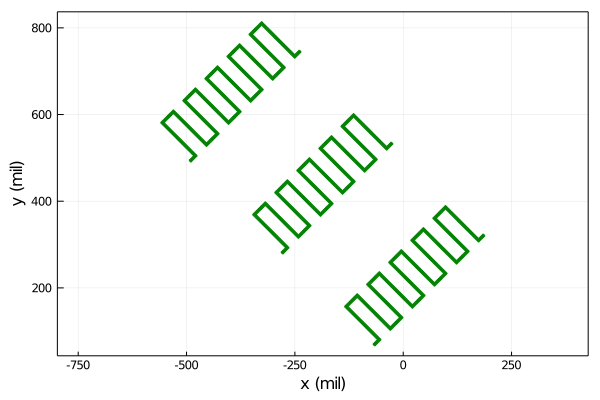
\includegraphics[scale=0.5,trim=150 50 100 20,clip=true]{meanderlines.png} \qquad \quad
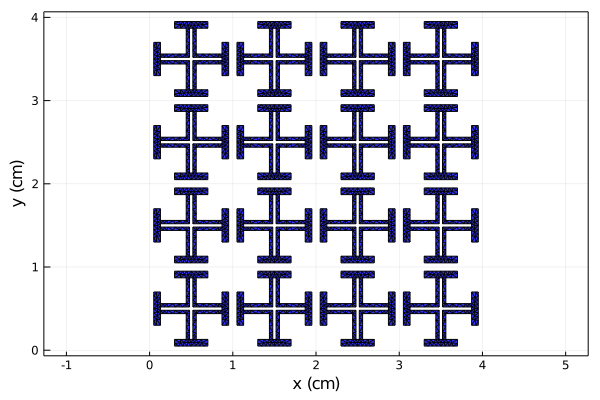
\includegraphics[scale=0.5,trim=150 50 100 20,clip=true]{jcrossarray.png}
}

\vspace{1.5in}

This document is licensed under the Creative Commons Attribution 4.0 International License.
To view a copy of this license, visit \url{http://creativecommons.org/licenses/by/4.0/}
or send a letter to Creative Commons, PO Box 1866, Mountain View, CA 94042, USA. 


% \begin{abstract}
% \lipsum[1-2]
% \end{abstract}

\clearpage

\tableofcontents*
\clearpage


\chapter{Introduction}
These notes constitute the theory documentation for the \pssfss\
program.  \pssfss\ is a \href{https://julialang.org/}{Julia} \cite{bezanson2017julia} program for the analysis
of polarization and frequency selective surfaces (PSSs and FSSs). The
structure under consideration may contain any number of 
stratified dielectric \emph{layers}, possibly including one or more
zero-thickness conducting\footnote{imperfect conductors 
are also allowed} \emph{sheets} located at the dielectric interface
layers.  The metalization pattern on the sheets is 
assumed to exhibit a two-dimensional periodicity, which may vary from
sheet to sheet.  The structure is illuminated by 
a monochromatic plane wave incident at an arbitrary angle, and the
goal of this analysis is to efficiently compute the complex scattering
matrix whose entries are reflection and transmission coefficients for
the scattered plane waves.  Various performance parameters can be obtained
from the scattering matrix, such as reflection and transmission
coefficients, axial ratio, polarization purity, delta insertion phase
delay, etc.  

To calculate the fields scattered from the metallic sheets, we will
use one of two approaches, depending on the sheet geometry:
\begin{enumerate}
\item If a sheet's unit cell of periodicity is mostly absent of
  metalization (``wire'', ``strip'', or ``capacitive'' type FSSs are
  typical examples of this), 
  it is more efficient to replace the metalization
  with unknown induced electric surface current, which will be
  solved for in the course of the analysis.
\item Alternatively, if the unit cell is mostly metalized (as in a
  ``slot'' or ``inductive'' type of FSS), then it is
  more efficient to solve for the tangential electric field in the
  non-metalized (``void'') area.  In practice this is done by filling
  in the void regions 
  with metalization and impressing upon these regions induced
  (fictitious) magnetic surface current.  Note that this technique can
  only be used when the metalization is assumed to be perfectly
  conducting.  Lossy conducting metalization requires the use of
  electric surface currents.
\end{enumerate}

The unknown electric or magnetic surface currents in the unit cell are
approximately determined by solving a mixed-potential integral
equation using
the method of moments in conjunction with the so-called ``RWG''
triangle subdomain basis functions \cite{rawg:82}. 

Each sheet in the structure is characterized by its generalized
scattering matrix (GSM).  ``Generalized'' refers to the fact that both
propagating and evanescent modes are treated.  The GSMs of the sheets
and dielectric layers are cascaded to obtain the GSM of the entire
structure. If the sheets do not all share the same periodic lattice,
then the sheet interactions are approximated by accounting only for
the dominant, propagating TE and TM modes during the cascading
process.  Also, if a sheet is surrounded by very thin dielectric
layers, then it would require a very large number of evanescent modes
to correctly model the effects of these layers.  So in this case, the
composite GSM of the sheet together with its surrounding thin layers
is directly computed, by
using a Green's function for multiply stratified dielectric layers.

This document is organized as follows:
\begin{description}[align=left]
  \item[Chapter~\ref{chap:fund}] documents the basic assumptions and
  fundamental equations for the fields and potentials needed in the
  rest of the analysis.
  \item[Chapter~\ref{chap:periodicity}] describes the type of
  periodic structures treated in this analysis, defines the direct and
  reciprocal lattices, and derives the form of Floquet modes used in
  subsequent chapters.
  \item[Chapter~\ref{chap:gsm}] defines the generalized 
  scattering matrix (GSM), and derives formulas for the GSMs of
  canonical structures needed later in the analysis.
  \item[Chapter~\ref{chap:mpgf}] derives an efficient, wide-band
  formula for the potential Green's functions for abutted half-spaces
  under quasi-periodic (Floquet) boundary conditions, as needed for
  FSS and PSS sheets that are surrounded by reasonably thick adjacent
  dielectric layers.
  \item[Chapter~\ref{chap:gfstratified}] extends this formulation to
  multiply stratified media on each side of the sheet, as is needed for
  a sheet immediately adjacent to one or more very thin dielectric
  layers.
  \item[Chapter~\ref{chap:incgsm}] discusses how to calculate the
  incident fields and extract scattering matrix entries from computed 
  currents.
  \item[Chapter~\ref{chap:mom}] provides the details of the method of
    moments (MoM) solution of the mixed potential integral equations for  
    the electric or magnetic currents flowing on the FSS/PSS sheets.
    Care is taken to exploit the wide-band nature of the Green's
    functions to minimize matrix fill time for multi-frequency
    analysis.
  \item[Chapter~\ref{chap:performance}] describes the performance parameters
      that are available as output of the program.
\end{description}


\mainmatter

\include{chapter1}
\include{chapter2}
\include{chapter3}
\include{chapter4}
\include{chapter5}
\include{chapter6}
\include{chapter7}
\include{chapter8}



\appendix
\renewcommand{\theequation}{\Alph{chapter}.\arabic{equation}}

\chapter{Orthogonality of Floquet Modes}

\label{app:orthogonal}
We wish to show that the Floquet modes are orthogonal in the following
sense:
\begin{equation}
  \label{eq:apmain}
  \iint_{U'}
  \e_{pmn} \cross \h_{p'm'n'}^* \bdot \z \; \d A  
    = \delta_{pp'} \delta_{mm'} \delta_{nn'} P_{pmn} 
\end{equation}
where $U'$ is the restriction of the unit cell to the plane $z=0$,
$\e_{pmn}$ and $\h_{p'm'n'}$ are defined in
Equations~\eqref{eq:modaldefs}, 
$\delta_{kl}$ is the Kronecker delta, and $P_{pmn}$ 
is given in Equation~\eqref{eq:Ppmn}.
Verification of Equation~\eqref{eq:apmain} is treated in two cases:



\section{Both Modes Share Common Wave Vector}
We consider here the case with 
$\vecbeta_{mn}= \vecbeta_{m'n'}$
which implies that
\begin{equation}
  m\vecbeta_1 + n\vecbeta_2 = m'\vecbeta_1 + n'\vecbeta_2.
  \label{eq:equalbeta}
\end{equation}
Taking the cross product of each side of \eqref{eq:equalbeta} with
$\vecbeta_1$ shows that $n=n'$, and similarly, crossing both sides
with $\vecbeta_2$ shows that $m=m'$.
It remains to show orthogonality when $p\neq p'$ and also
that the normalization given in Equation~\eqref{eq:apmain} is
correct when $p=p'$.  These both follow immediately from examining
Equations~\eqref{eq:modaldefs}, after noting that 
\begin{itemize}
\item The cross product 
  $\e_{pmn} \cross \h_{p'mn}^*$ is identically zero for $p\neq p'$ 
  at all points in the unit cell due to colinearity of the two vectors,
  and
\item The phase variation of the two factors in the cross product
  perfectly cancel.
\end{itemize}


\section{Distinct Wave Vectors}
Here we assume that the two wave vectors $\vecbeta_{mn}$ and
$\vecbeta_{m'n'}$ are distinct.  Orthogonality then depends on
the value of the integral
\begin{equation}
 I_{mnm'n'} \equiv \iint_{U'} \mkern -5mu
  e^{-j(\vecbeta_{mn} - \vecbeta_{m'n'}) \bdot \vecrho} \, \d A
  =
  \iint_{U'} \mkern -5mu
  e^{-j[(m-m')\vecbeta_1 + (n-n')\vecbeta_2] \bdot \vecrho} \, \d A.
\label{eq:zerointegral}
\end{equation}
We introduce the change of variables $\vecrho = \xi_1\s_1 + \xi_2\s_2$
so that the area element is $\d A = A \, \d \xi_1 \, \d \xi_2$, where $A
= \z \bdot \s_1 \cross \s_2$ is the transverse area of the unit cell.
The integral in \eqref{eq:zerointegral} then becomes
\begin{equation}
 I_{mnm'n'}=  A  \int_{\xi_1=0}^{1} \int_{\xi_2=0}^{1} \mkern -5mu
  e^{-j[(m-m')\vecbeta_1 + (n-n')\vecbeta_2] \bdot
  (\xi_1\s_1+\xi_2\s_2)} \, \d \xi_1 \, \d \xi_2
\end{equation}
We now employ the properties of the direct and reciprocal lattice
vectors:
\begin{subequations}
  \begin{align}
    \vecbeta_1\bdot\s_1 &= 2\pi, \quad \vecbeta_1\cdot\s_2 = 0 \\
    \vecbeta_2\bdot\s_2 &= 2\pi, \quad \vecbeta_2\cdot\s_1 = 0.
  \end{align}
\end{subequations}
The integral then becomes
\begin{align}
  I_{mnm'n'} &= A \int_{\xi_1=0}^{1} \int_{\xi_2=0}^{1} \mkern -5mu
   e^{-j2\pi[(m-m')\xi_1 + (n-n')\xi_2]} \, \d \xi_1 \, \d \xi_2
   \nonumber \\
   &= A e^{-j(m-m')\pi} e^{-j(n-n')\pi} j_0[(m-m')\pi] j_0[(n-n')\pi]
   \nonumber \\
   &= A e^{-j(m-m')\pi} e^{-j(n-n')\pi} \delta_{mm'} \delta_{nn'}
   \nonumber \\
   &= A \delta_{mm'} \delta_{nn'},
\end{align}
where we have used the identity 
\begin{equation}
  \int_{0}^1 e^{-j2\pi\alpha x} \d x = e^{-j\alpha\pi} j_0(\alpha\pi),
\end{equation}
$j_0$ being the spherical Bessel function of the first kind of order
zero:
\begin{equation}
  j_0(x) = 
  \begin{cases}
    \frac{\sin x}{x} & \text{if $x \neq 0$} \\
    1 & \text{if $x=0$}.
  \end{cases}
\end{equation}
This completes the orthogonality proof.



\chapter{\label{app:singint}Evaluation of Singular Integrals}
 This Appendix is concerned with evaluating the singular integrals 
 that occur in 
 Equations~\eqref{eq:Aiuv2} and \eqref{eq:Phiiuv2}.  Since we are concerned
 only with strictly planar structures, both integrals can be simply
 evaluated by specializing the formulas of \cite{wrgs:84} to the case where
 the observation point is in the plane of the source triangle.
 
 The two integrals of interest are
 \begin{align}
   \iint_{T^v} \frac{\d S'}{\norm{\r' - \r^{cu}}} \;\;\;\; \text{and} \;\;\;\;
   \iint_{T^v} \frac{\r'-\r_i}{\norm{\r' - \r^{cu}}} \, \d S'
   \label{eq:twoints}
 \end{align}
 where $T^v$ is the source triangle, and $\r^{cu}$ is the centroid of the observation 
 triangle.  For the purposes of this Appendix we adopt a local numbering scheme 
 $\r_i \in \{\r_1,\r_2,\r_3\}$ for the source triangle vertices.  For convenience in the
 formulas presented below, we also define $\r_4 \equiv \r_1$.
 
 The second, vector, integral in \eqref{eq:twoints} can be written
 \begin{equation}
   \iint_{T^v} \frac{\r'-\r_i}{\norm{\r' - \r^{cu}}} \, \d S' =
   \iint_{T^v} \frac{\r'-\r^{cu}}{\norm{\r' - \r^{cu}}} \, \d S' +
   (\r^{cu} - \r_i) \iint_{T^v} \frac{\d S'}{\norm{\r' - \r^{cu}}}
 \end{equation}
 which is a more convenient representation, because it is now
 expressed in terms of the two integrals directly treated in \cite{wrgs:84}.
 We thus have the two formulas
 \begin{subequations}
   \label{eq:cfint}
   \begin{align}
     \iint_{T^v} \frac{\d S'}{\norm{\r' - \r^{cu}}} &= 
     \sum_{i=1}^{3} \P_i^0 \bdot \u_i \ln \frac{P_i^+ + l_i^+}{P_i^- + l_i^-} \\
     \iint_{T^v} \frac{\r'-\r^{cu}}{\norm{\r' - \r^{cu}}} \, \d S' &=
     \frac{1}{2} \sum_{i=1}^{3} \u_i 
     \left[
       \left( P_i^0 \right)^2 
       \ln \frac{P_i^+ + l_i^+}{P_i^- + l_i^-}
       + l_i^+ P_i^+ - l_i^- P_i^-
     \right]
 \end{align} 
\end{subequations}
\noindent
which are the specializations of Equations~(5) and (6), respectively, of 
\cite{wrgs:84} to the case when the variable $d$ defined in \cite{wrgs:84}
is zero.  The additional variables needed to evaluate \eqref{eq:cfint} are
\begin{subequations}
\begin{align}
  \l_i &= \r_{i+1} - \r_i, & l_i &= \norm{\l_i}, & \lhat_i &= \l_i / l_i, \\
  l_i^+ &= (\r_{i+1} - \r^{cu}) \bdot \lhat_i, & 
  l_i^- &= (\r_{i} - \r^{cu}) \bdot \lhat_i, &
  \u_i &= \lhat_i \cross \n, \\
  \n &= \frac{(\r_3-\r_2)\cross(\r_1-\r_2)}{2A^v}, &
  \P_i^0 &= (\r_i - \r^{cu}) - l_i^- \lhat, &
  P_i^0 &= \norm{\P_i^0}, \\
  P_i^+ &= \norm{\r_{i+1} - \r^{cu}}, &  P_i^- &= \norm{\r_{i} - \r^{cu}}
\end{align}
\end{subequations}


\chapter{Basis Function Inner Products\label{ap:ip}}
This appendix is concerned with computing the inner product of two basis
functions $\innerprod{\f_n, \f_m}$.  Clearly, the inner product is nonzero 
only when the support of basis functions $m$ and $n$ are common to at 
least a single triangle.  The  
two cases to be treated are when $m=n$, or $m \neq n$.
\subsection{Basis Function Self Inner Product\label{sec:ipself}}
Using the definition of Equation (\ref{eq:basis}) we have
\begin{equation}
  \innerprod{\f_n, \f_n} = B^+ + B^-
\end{equation}
where
\begin{equation}
  B^{\pm} = \frac{l_n^2}{4{A_n^{\pm}}^2} \iint_{T_n^{\pm}} 
                \vecrho_n^{\pm} \cdot \vecrho_n^{\pm} \; dS.  \label{eq:Bpm}
\end{equation}
As shown in Figure \ref{fig:selfip} 
\begin{figure}
  \setlength{\unitlength}{0.25 in}
  \begin{center}
  \begin{picture}(16,6)(0,2)
    \thicklines
    \put(3,3){\vector(1,0){4}}
    \put(3,3){\vector(1,1){4}}
    \put(7,7){\vector(2,-1){4}}
    \put(7,3){\vector(2,1){4}}
    %
    \put(5,3.6){\makebox(0,0){$T_n^+$}}
    \put(8.5,5){\makebox(0,0){$T_n^-$}}
    \put(5,2.6){\makebox(0,0)[t]{$\l_a^+$}}
    \put(9,3.6){\makebox(0,0)[t]{$\l_a^-$}}
    \put(5,5.2){\makebox(0,0)[b]{$\l_b^+$}}
    \put(9,6.2){\makebox(0,0)[b]{$\l_b^-$}}
    \thinlines
    \put(7,3){\line(0,1){4}}
    \put(6.8,5){\makebox(0,0)[r]{$l_n$}}
  \end{picture}
  \end{center}
  \caption{Geometry for calculating self-term inner product.}
  \label{fig:selfip}
\end{figure}
let $\l_a^{+}$ and $\l_b^{+}$ be 
vectors drawn from the free vertex (i.e. the vertex which is not incident upon 
edge $l_n$) of triangle $T_n^{+}$ to the nodes of
edge $n$.   Vectors $\l_a^{-}$ and $\l_b^-$ are defined similarly for triangle 
$T_n^-$ except that they are directed towards the free vertex.
Using normalized area coordinates we can then write 
$\vecrho_n^{\pm}$ as
\begin{equation}
  \vecrho_n^{\pm} = \xi \l_a^{\pm} + \eta \l_b^{\pm}.
\end{equation}
Equation (\ref{eq:Bpm}) can now be evaluated as
\begin{align}
  B^{\pm} &= \frac{l_n^2}{4{A_n^{\pm}}^2}  \int_0^1 \int_0^{1-\eta}
  \!\!\!
  (\xi\l_a^{\pm} + \eta\l_b^{\pm}) \bdot
  (\xi\l_a^{\pm} + \eta\l_b^{\pm}) \,
  (2 A_n^{\pm} \, \d\xi\, \d\eta )              \nonumber \\
  &= \frac{l_n^2}{2A_n^{\pm}}  \int_0^1 \int_0^{1-\eta}
  \!\!\!
  (\xi^2 {l_a^{\pm}}^2 + \eta^2 {l_b^{\pm}}^2 + 2\xi\eta
  \l_a^{\pm} \bdot \l_b^{\pm}) \, \d\xi \, \d\eta \nonumber \\
  &= \frac{l_n^2}{24A_n^{\pm}}
  ({l_a^{\pm}}^2 + {l_b^{\pm}}^2 + \l_a^{\pm} \bdot \l_b^{\pm}) \nonumber \\
  &= \frac{l_n^2}{48A_n^{\pm}}
  (3{l_a^{\pm}}^2 + 3{l_b^{\pm}}^2 - l_n^2).
\end{align}
The final equality above follows from the Law of Cosines:
\begin{equation}
  \l_a^{\pm} \cdot \l_b^{\pm} = \frac{1}{2} ( {l_a^{\pm}}^2 +{l_b^{\pm}}^2
                                               - l_n^2 ).
\end{equation}
Although the above result assumed that the two triangles comprising
the support of $\f_n$ are
adjacent, the derivation is identical in the case where they are separated.
\subsection{Inner Product of Distinct Basis Functions}
We denote the triangle common to basis functions $m$ and $n$ as
$T^{mn}$.  The vertices 
are denoted by $\r_a$, $\r_b$, and $\r_c$, where without loss of 
generality we assume,
as shown in Figure \ref{fig:ipdiff}, that $\r_a$ is opposite the
center edge of basis function $m$ and 
\begin{figure}
  \setlength{\unitlength}{0.25 in}
  \begin{center}
  \begin{picture}(8,6)
    \thicklines
    \put(2,2){\line(1,0){4}}
    \put(2,2){\line(1,1){2}}
    \put(4,4){\line(1,-1){2}}
    %
    \put(4,4.2){\makebox(0,0)[b]{$\r_a$}}
    \put(2,1.8){\makebox(0,0)[t]{$\r_b$}}
    \put(6,1.8){\makebox(0,0)[t]{$\r_c$}}
    \put(4,1.8){\makebox(0,0)[t]{$m$}}
    \put(5.2,3.1){\makebox(0,0)[b]{$n$}}
    \put(4,3){\makebox(0,0)[t]{$T^{mn}$}}
    \put(2,2){\circle*{.15}}
    \put(4,4){\circle*{.15}}
    \put(6,2){\circle*{.15}}
  \end{picture}
  \end{center}
  \caption{Geometry for calculating inner product of distinct basis 
           functions.}
  \label{fig:ipdiff}
\end{figure}
$\r_b$ is opposite the center edge of basis function $n$.  
We also define $\l_{ij} = \r_i - \r_j$, for 
$i,j \in \{a,b,c\}$.  Then
\begin{equation}
  \innerprod{\f_n, \f_m} = \pm \frac{l_{ac}l_{bc}}{4(A^{mn})^2}
  e^{j(\theta_n-\theta_m)}
        \iint_{T^{mn}} \!\!\!\!\!\!
        (\r - \r_b) \bdot (\r - \r_a) \, \d S.
\end{equation}
The negative sign above is used if one of the basis functions $\f_n$ or $\f_m$ 
defines positive current to flow out of the triangle while the other basis 
function defines positive current to flow into the triangle.  If the two basis 
functions agree in this respect the positive sign is used.  Using normalized 
area coordinates the factors in the integral can be written
\begin{equation}
  \r - \r_a = \xi \l_{ba} + \eta \l_{ca}
\end{equation}
\begin{equation}
  \r - \r_b = (\r-\r_a) + (\r_a - \r_b) = \xi \l_{ba} + \eta \l_{ca} + 
                                  \l_{ab}.
\end{equation}
The inner product can now be written as the phase factor times the 
sum of two terms
\begin{equation}
  \innerprod{\f_n, \f_m} = \pm (C_1 + C_2) e^{j(\theta_n-\theta_m)}
\end{equation}
 where
\begin{equation}
  C_1 =  \frac{l_{ac}l_{bc}}{2A^{mn}}\int_0^1 \int_0^{1-\eta}
  \!\!\!\!\!
              (\xi\l_{ba} + \eta\l_{ca}) \bdot
              (\xi\l_{ba} + \eta\l_{ca})  \, \d\xi\, \d\eta  
\end{equation}
and
\begin{equation}
  C_2 =  \frac{l_{ac}l_{bc}}{2A^{mn}}\int_0^1 \int_0^{1-\eta}
  \!\!\!\!\!  \l_{ab}  \bdot
              (\xi\l_{ba} + \eta\l_{ca})  \, \d\xi\, \d\eta  
\end{equation}
$C_1$ is easily found using the results of Section \ref{sec:ipself}:
\begin{equation}                                  
  C_1 = \frac{l_{ac}l_{bc}}{48A^{mn}}
       (3l_{ab}^2 + 3l_{ac}^2 - l_{bc}^2).
\end{equation}
An expression for $C_2$ is also obtained with a bit of algebra:
\begin{align}
  C_2 &= \frac{l_{ac}l_{bc}}{2A^{mn}}\int_0^1 \int_0 ^{1-\eta}
  \!\!\!\!\!
           (-\xi l_{ab}^2 + \eta \l_{ab} \cdot \l_{ca} ) \, \d\xi \, \d\eta
                   \nonumber \\
       &=  \frac{l_{ac}l_{bc}}{12A^{mn}} ( \l_{ab} \cdot \l_{ca} - l_{ab}^2)
                   \nonumber \\
       & =  \frac{l_{ac}l_{bc}}{24 A^{mn}} (l_{bc}^2 - 3l_{ab}^2 - l_{ac}^2)
\end{align}
where the last equality follows from the Law of Cosines.

Combining the expressions for $C_1$ and $C_2$ yields
\begin{equation}
  \innerprod{\f_n,\f_m} = \pm e^{j(\theta_n-\theta_m)}
  \frac{l_{ac}l_{bc}}{48A^{mn}}(l_{ac}^2+l_{bc}^2 
                               - 3 l_{ab}^2)
\end{equation}
which is the desired formula.



\backmatter

%%% BIBLIOGRAPHY
%%% -------------------------------------------------------------

\bibliographystyle{ieeetr}
\bibliography{pssfss.bib}

\end{document}
